\begin{figure}[htbp]
\centering
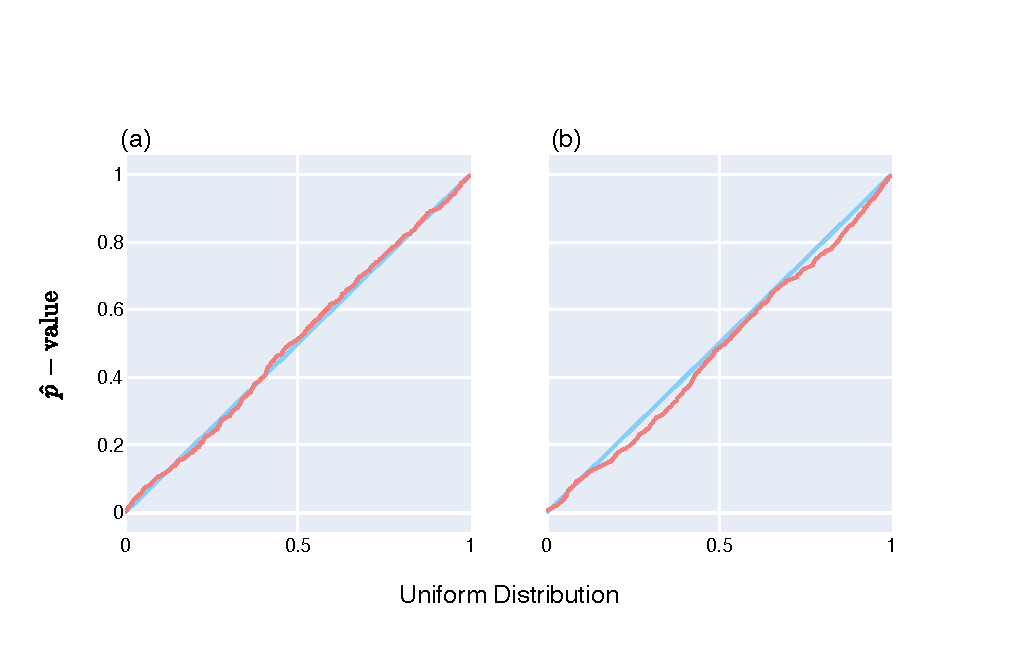
\includegraphics[width=\textwidth]{figures/plots/synthetic/adj-temp_eop/High JSD, High Entropy.pdf}
\caption[Both equivalence of process tests were consistent with theoretical approximations]{\textbf{Both equivalence of process tests were consistent with theoretical approximations.} The Quantile-Quantile plots compare the distribution of $\hat p-$values (pink line) to the uniform distribution (blue line). (a) $\hat p-$values from temporal equivalence of process, (b) $\hat p-$values from adjacent equivalence of process. Each data set contains 1,000 synthetic stationary alignments. This result is shown for 300bp alignments generated by the High JSD, High Entropy seed. The result were comparable for all seeds and all length (see Figure \ref{fig:synthetic/adj_eop/all_seeds} and \ref{fig:synthetic/temp_eop/all_seeds}).}
\label{fig:synthetic/adj-temp_eop/HighJSDHighEntropy}
\end{figure}